% Emacs, this is -*-latex-*-

\ex{Visualizando e analisando distribui\'c\~oes de Gibbs via grafos n\~ao direcionados}
\label{ex:visualising-gibbs-distributions}
Consideramos aqui a distribui\'c\~ao de Gibbs
$$p(x_1, \ldots, x_5) \propto \phi_{12}(x_1,x_2)\phi_{13}(x_1,x_3)\phi_{14}(x_1,x_4)\phi_{23}(x_2,x_3)\phi_{25}(x_2,x_5)\phi_{45}(x_4,x_5)$$

\begin{exenumerate}
    \item Visualize-a como um grafo n\~ao direcionado.
    
    \begin{solution}
        Desenhamos um n\'o para cada vari\'avel aleat\'oria $x_i$. Existe uma aresta entre dois n\'os se as vari\'aveis correspondentes co-ocorrem em um fator.
        \begin{center}
            \scalebox{0.9}{
                \begin{tikzpicture}[ugraph]
                    
                    \node[cont] (x1) at (0,0) {$x_1$};
                    \node[cont] (x2) at (2,1) {$x_2$};
                    \node[cont] (x3) at (1,2) {$x_3$};
                    \node[cont] (x4) at (4,0) {$x_4$};
                    \node[cont] (x5) at (3,2) {$x_5$};
                    
                    \draw(x1) -- (x2);
                    \draw(x1) -- (x3);
                    \draw(x1) -- (x4);
                    \draw(x2) -- (x3);
                    \draw(x2) -- (x5);
                    \draw(x4) -- (x5);
                    
            \end{tikzpicture}}
        \end{center}
        
    \end{solution}
    
    \item Quais s\~ao os vizinhos de $x_3$ no grafo?
    
    \begin{solution}
        Os vizinhos s\~ao todos os n\'os para os quais existe uma \'unica aresta de conex\~ao. Assim:
        $\ne(x_3) = \{x_1, x_2\}$. (Note que, s\^o vezes, podemos denotar $\ne(x_3)$ por $\ne_3$.)
    \end{solution}
    
    \item Temos $x_3 \independent x_4 \mid x_1, x_2$?
    
    \begin{solution}
        Sim. O conjunto de condicionamento $\{x_1,x_2\}$ \'e igual a $\ne_3$, que tamb\'em \'e o Markov blanket de $x_3$. Isso significa que $x_3$ \'e condicionalmente independente de todas as outras vari\'aveis dado $\{x_1,x_2\}$, i.e.\ $x_3 \independent x_4,x_5 \mid x_1, x_2$, o que implica que $x_3 \independent x_4 \mid x_1, x_2$. (Tamb\'em \'e poss\'ivel usar a separa\'c\~ao de grafos para responder \`a quest\~ao.)
    \end{solution}
    
    \item Qual \'e o Markov blanket de $x_4$?
    
    \begin{solution}
        O Markov blanket de um n\'o em um modelo gr\'afico n\~ao direcionado \'e igual ao conjunto de seus vizinhos: $\MB(x_4) = \ne(x_4) = \ne_4 = \{x_1,x_5\}$. Isso implica, por exemplo, que
        $x_4 \independent x_2,x_3 \mid x_1,x_5$.
    \end{solution}
    
    \item Em qual conjunto m\'inimo de vari\'aveis $A$ precisamos condicionar para ter $x_1 \independent x_5 \mid A$?
    
    \begin{solution}
        Primeiro identificamos todas as trilhas de $x_1$ para $x_5$. Existem tr\^es dessas trilhas: $(x_1,x_2,x_5)$, $(x_1, x_3, x_2, x_5)$, e $(x_1,x_4, x_5)$. Condicionar em $x_2$ bloqueia as duas primeiras trilhas, condicionar em $x_4$ bloqueia a \'ultima. Temos, portanto: $x_1 \independent x_5 \mid x_2,x_4$, de modo que $A=\{x_2,x_4\}$.
    \end{solution}
    
\end{exenumerate}

% --------------------------------------------------

\ex{Fatoriza\'c\~ao e independ\^encias para modelos gr\'aficos n\~ao direcionados}
\label{ex:factorisation-independencies-undirected-graphical-model}
Considere o modelo gr\'afico n\~ao direcionado definido pelo grafo na Figura \ref{fig:undirected-graphical-model}.
\begin{figure}[h]
    \begin{center}
        \scalebox{0.9}{ % x,y
            \begin{tikzpicture}[ugraph]
                \node[cont] (x1) at (0,0) {$x_1$};
                \node[cont] (x2) at (0,-2) {$x_2$};
                \node[cont] (x3) at (2,0) {$x_3$};
                \node[cont] (x4) at (2,-2) {$x_4$};
                \node[cont] (x5) at (3,-1) {$x_5$};
                \node[cont] (x6) at (5,-2) {$x_6$};
                \draw(x1) -- (x3);
                \draw(x1) -- (x2);
                \draw(x2) -- (x4);
                \draw(x1) -- (x4);
                \draw(x3) -- (x4);
                \draw(x3) -- (x5);
                \draw(x4) -- (x5);
                \draw(x5) -- (x6);
                \draw(x4) -- (x6);
        \end{tikzpicture}}
    \end{center}
    \caption{\label{fig:undirected-graphical-model} Grafo para o \exref{ex:factorisation-independencies-undirected-graphical-model}}
\end{figure}

\begin{exenumerate}
    
    
    \item Qual \'e o conjunto de distribui\'c\~oes de Gibbs que \'e induzido pelo grafo?
    
    \begin{solution}
        O grafo na Figura \ref{fig:undirected-graphical-model} possui quatro cliques m\'aximos:
        $$(x_1,x_2,x_4) \quad (x_1,x_3,x_4) \quad (x_3,x_4,x_5) \quad (x_4, x_5, x_6)$$
        As distribui\'c\~oes de Gibbs s\~ao, portanto,
        $$p(x_1,\ldots,x_6) \propto \phi_1(x_1,x_2,x_4) \phi_2(x_1,x_3,x_4) \phi_3(x_3,x_4,x_5) \phi_4(x_4, x_5, x_6)$$
    \end{solution}
    
    \item Seja $p$ uma fdp que se fatoriza de acordo com o grafo. A rela\'c\~ao $p(x_3 | x_2, x_4) = p(x_3 | x_4)$ se sustenta?
    
    \begin{solution}
        $p(x_3 | x_2, x_4) = p(x_3 | x_4)$ significa que $x_3 \independent
        x_2 \mid x_4$. Podemos usar o grafo para verificar se isso
        geralmente se sustenta para fdps que se fatorizam de acordo com o
        grafo. Existem m\'ultiplas trilhas de $x_3$ para $x_2$, incluindo
        a trilha $(x_3,x_1,x_2)$, que n\~ao \'e bloqueada por $x_4$. A partir do
        grafo, n\~ao podemos, portanto, concluir que $x_3 \independent x_2 \mid x_4$,
        e $p(x_3 | x_2, x_4) = p(x_3 | x_4)$ geralmente n\~ao valer\'a
        (a rela\'c\~ao pode valer para alguns fatores $\phi_i$ cuidadosamente definidos).
        
    \end{solution}
    
    \item Explique por que $x_2 \independent x_5 \mid x_1,x_3,x_4,x_6$ vale para todas as distribui\'c\~oes que se fatorizam sobre o grafo.
    
    \begin{solution}
        Distribui\'c\~oes que se fatorizam sobre o grafo satisfazem a propriedade de Markov em pares. Como $x_2$ e $x_5$ n\~ao s\~ao vizinhos, e $x_1,x_3,x_4,x_6$
        s\~ao os n\'os restantes no grafo, a rela\'c\~ao de independ\^encia segue da propriedade de Markov em pares.
    \end{solution}
    
    \item Suponha que voc\^e gostaria de aproximar $\E (x_1 x_2 x_5 \mid
    x_3,x_4)$, i.e.\ o valor esperado do produto de $x_1$, $x_2$,
    e $x_5$ dados $x_3$ e $x_4$, com uma m\'edia amostral. Voc\^e
    precisa ter observa\'c\~oes conjuntas para todas as cinco vari\'aveis $x_1, \ldots, x_5$?
    
    \begin{solution}
        
        No grafo, todas as trilhas de $\{x_1,x_2\}$ para $x_5$ s\~ao bloqueadas por $\{x_3,x_4\}$, de modo que $x_1, x_2 \independent x_5 \mid x_3, x_4$. Temos, portanto,
        $$\E (x_1 x_2 x_5 \mid x_3,x_4) =  \E (x_1 x_2 \mid x_3,x_4)  \E (x_5 \mid x_3,x_4).$$
        Assim, precisamos apenas de observa\'c\~oes conjuntas de $(x_1, x_2, x_3, x_4)$ e $(x_3, x_4,x_5)$. As vari\'aveis $(x_1,x_2)$ e $x_5$ n\~ao precisam ser medidas conjuntamente.
        
    \end{solution}
    
\end{exenumerate}


% -----------------------------------------
\ex{Fatoriza\'c\~ao e independ\^encias para modelos gr\'aficos n\~ao direcionados}
\label{ex:factorisation-independencies-diamond}

Considere o modelo gr\'afico n\~ao direcionado definido pelo seguinte grafo, s\^o vezes chamado de configura\'c\~ao em diamante.

\begin{center}
    \scalebox{1}{ % w,x,y,z
        \begin{tikzpicture}[ugraph]
            \node[cont] (w) at (0,1) {$w$};
            \node[cont] (x) at (1,2) {$x$};
            \node[cont] (y) at (2,1) {$y$};
            \node[cont] (z) at (1,0) {$z$};
            \draw(w) -- (x);
            \draw(w) -- (z);
            \draw(x) -- (y);
            \draw(y) -- (z);
        \end{tikzpicture}
    }
\end{center}

\begin{exenumerate}
    
    \item Como as fdps/fmps do modelo gr\'afico n\~ao direcionado se fatorizam?
    
    \begin{solution}
        Os cliques m\'aximos s\~ao $(x, w)$, $(w, z)$, $(z, y)$ e $(x,
        y)$. O modelo gr\'afico n\~ao direcionado consiste, portanto, de fdps/fmps
        que se fatorizam da seguinte forma
        \begin{equation}
            p(x, w, z, y) \propto \phi_1(x,w) \phi_2(w,z) \phi_3(z,y) \phi_4(x,y)
        \end{equation}
        
    \end{solution}
    
    \item Liste todas as independ\^encias que valem para o modelo gr\'afico n\~ao direcionado.
    
    \begin{solution}
        Podemos gerar as independ\^encias condicionando em
        conjuntos progressivamente maiores. Como existe uma trilha entre quaisquer dois
        n\'os, n\~ao h\'a independ\^encias n\~ao condicionais. Se condicionarmos em
        uma \'unica vari\'avel, ainda haver\'a uma trilha que conecta as
        restantes. Consideremos, ent\~ao, o caso em que condicionamos em
        dois n\'os. Pela separa\'c\~ao de grafos, temos
        \begin{equation}
            w \independent y \mid x,z \quad \quad x \independent z \mid w,y
        \end{equation}
        Estas s\~ao todas as independ\^encias que valem para o modelo, j\'a que
        condicionar em tr\^es n\'os n\~ao leva a nenhuma independ\^encia em
        um modelo com quatro vari\'aveis.
    \end{solution}
    
    
\end{exenumerate}

% --------------------------------------------------

\ex{Fatoriza\'c\~ao a partir dos Markov blankets I}
\label{ex:factorisation-from-the-Markov-blankets-I}

Suponha que voc\^e conhe\'ca os seguintes Markov blankets para todas as vari\'aveis $x_1,
\ldots, x_4, y_1, \ldots y_4$ de uma fdp ou fmp $p(x_1, \ldots, x_4,
y_1, \ldots,y_4)$.
\begin{align}
    \MB(x_1) &= \{x_2, y_1\} & \MB(x_2)&=\{x_1, x_3, y_2\} & \MB(x_3)&=\{x_2, x_4, y_3\} & \MB(x_4)&=\{x_3, y_4\}\\
    \MB(y_1) &= \{x_1\}      & \MB(y_2)&= \{x_2\}          &  \MB(y_3)&= \{x_3\}          &  \MB(y_4) &= \{x_4\}
\end{align}
Assumindo que $p$ \'e positiva para todos os valores poss\'iveis
de suas vari\'aveis, como $p$ se fatoriza?

\begin{solution}
    Em modelos gr\'aficos n\~ao direcionados, o Markov blanket para uma vari\'avel \'e
    o mesmo que o conjunto de seus vizinhos. Assim, quando nos s\~ao dados todos os
    Markov blankets, sabemos qual propriedade de Markov local $p$ deve
    satisfazer. Para distribui\'c\~oes positivas, temos uma equival\^encia entre $p$
    satisfazendo a propriedade de Markov local e $p$ se fatorizando sobre o
    grafo. Portanto, para especificar a fatoriza\'c\~ao de $p$, basta
    construir o grafo n\~ao direcionado $H$ baseado nos Markov blankets e
    ent\~ao ler a fatoriza\'c\~ao.
    
    Precisamos construir um grafo onde os vizinhos de cada vari\'avel sejam iguais
    ao Markov blanket indicado. Isso pode ser feito facilmente come\'cando com
    um grafo vazio e conectando cada vari\'avel \`as vari\'aveis em seu
    Markov blanket.
    
    Vemos que cada $y_i$ est\'a apenas conectado a $x_i$. Incluindo esses
    Markov blankets, obtemos o seguinte grafo:
    
    \begin{center}
        \scalebox{1}{
            \begin{tikzpicture}[ugraph]
                \node[cont] (y1) at (0,0) {$y_1$};
                \node[cont] (y2) at (2,0) {$y_2$};
                \node[cont] (y3) at (4,0) {$y_3$};
                \node[cont] (y4) at (6,0) {$y_4$};
                \node[cont] (x1) at (0,2) {$x_1$};
                \node[cont] (x2) at (2,2) {$x_2$};
                \node[cont] (x3) at (4,2) {$x_3$};
                \node[cont] (x4) at (6,2) {$x_4$};
                \draw(x1)--(y1);\draw(x2)--(y2);\draw(x3)--(y3);\draw(x4)--(y4);
        \end{tikzpicture}}
    \end{center}
    
    Conectar os $x_i$ aos seus vizinhos de acordo com o Markov blanket resulta em:
    
    \begin{center}
        \scalebox{1}{
            \begin{tikzpicture}[ugraph]
                \node[cont] (y1) at (0,0) {$y_1$};
                \node[cont] (y2) at (2,0) {$y_2$};
                \node[cont] (y3) at (4,0) {$y_3$};
                \node[cont] (y4) at (6,0) {$y_4$};
                \node[cont] (x1) at (0,2) {$x_1$};
                \node[cont] (x2) at (2,2) {$x_2$};
                \node[cont] (x3) at (4,2) {$x_3$};
                \node[cont] (x4) at (6,2) {$x_4$};
                \draw(x1)--(y1);\draw(x2)--(y2);\draw(x3)--(y3);\draw(x4)--(y4);
                \draw(x1)--(x2);\draw(x2)--(x3);\draw(x3)--(x4);
        \end{tikzpicture}}
    \end{center}
    
    O grafo possui cliques m\'aximos de tamanho dois, a saber, os $x_i-y_i$ para
    $i=1,\ldots, 4$, e os $x_i-x_{i+1}$ para $i=1, \ldots, 3$. Dada
    a equival\^encia entre a propriedade de Markov local e a fatoriza\'c\~ao
    para distribui\'c\~oes positivas, sabemos que $p$ deve se fatorizar como
    \begin{align}
        p(x_1, \ldots, x_4, y_1, \ldots, y_4) = \frac{1}{Z} \prod_{i=1}^3 m_i(x_i,x_{i+1}) \prod_{i=1}^4 g_i(x_i,y_i),
    \end{align}
    onde $m_i(x_i, x_{i+1})>0$, $g(x_i,y_i)>0$ s\~ao fatores positivos (fun\'c\~oes de potencial).
    
    O modelo gr\'afico corresponde a uma vers\~ao n\~ao direcionada de um modelo oculto
    de Markov onde os $x_i$ s\~ao as vari\'aveis n\~ao observadas (latentes, ocultas)
    e os $y_i$ s\~ao as observadas. Note que os $x_i$
    formam uma cadeia de Markov.
    
\end{solution}

\ex{Fatoriza\'c\~ao a partir dos Markov blankets II}
\label{ex:factorisation-from-the-Markov-blankets-II}

Consideramos o mesmo cenário do Exerc\'icio \ref{ex:factorisation-from-the-Markov-blankets-I}, mas agora assumimos que n\~ao conhecemos todos os Markov blankets, mas apenas
\begin{align}
    \MB(x_1) &= \{x_2, y_1\} & \MB(x_2)&=\{x_1, x_3, y_2\} & \MB(x_3)&=\{x_2, x_4, y_3\} & \MB(x_4)&=\{x_3, y_4\}
\end{align}
Sem inserir mais independ\^encias do que aquelas especificadas pelos
Markov blankets, desenhe o grafo sobre o qual $p$ se fatoriza e apresente
a fatoriza\'c\~ao. (Novamente, assuma que $p$ \'e positiva para todos os valores
poss\'iveis de suas vari\'aveis).

\begin{solution}
    Adotamos a mesma abordagem do Exerc\'icio
    \ref{ex:factorisation-from-the-Markov-blankets-I}. Em particular, os
    Markov blankets de uma vari\'avel s\~ao seus vizinhos no grafo. Mas,
    como n\~ao nos s\~ao dados todos os Markov blankets e n\~ao temos permiss\~ao para
    inserir independ\^encias adicionais, devemos assumir que cada $y_i$ est\'a
    conectado a todos os outros $y$'s. Por exemplo, se n\~ao conect\'assemos
    $y_1$ e $y_4$, estar\'iamos afirmando a independ\^encia adicional $y_1
    \independent y_4 \mid x_1,x_2,x_3,x_4,y_2,y_3$.
    
    Temos, portanto, um grafo como segue:
    
    \begin{center}
        \scalebox{1}{
            \begin{tikzpicture}[ugraph]
                \node[cont] (y1) at (0,0) {$y_1$};
                \node[cont] (y2) at (2,0) {$y_2$};
                \node[cont] (y3) at (4,0) {$y_3$};
                \node[cont] (y4) at (6,0) {$y_4$};
                \node[cont] (x1) at (0,2) {$x_1$};
                \node[cont] (x2) at (2,2) {$x_2$};
                \node[cont] (x3) at (4,2) {$x_3$};
                \node[cont] (x4) at (6,2) {$x_4$};
                \draw(x1)--(y1);\draw(x2)--(y2);\draw(x3)--(y3);\draw(x4)--(y4);
                \draw(x1)--(x2);\draw(x2)--(x3);\draw(x3)--(x4);
                \draw(y1)--(y2);\draw(y1) to [bend right= 45] (y3);\draw(y1)  to [bend right= 45] (y4);
                \draw(y2)--(y3);\draw(y2) to [bend right=45]  (y4);\draw(y3)--(y4);
        \end{tikzpicture}}
    \end{center}
    
    A fatoriza\'c\~ao, portanto, \'e
    \begin{align}
        p(x_1, \ldots, x_4, y_1, \ldots, y_4) = \frac{1}{Z} g(y_1, \ldots, y_4) \prod_{i=1}^3 m_i(x_i,x_{i+1})\prod_{i=1}^4 g_i(x_i,y_i),
    \end{align}
    where the $m_i(x_i, x_{i+1})$, $g_i(x_i, y_i)$ and $g(y_1, \ldots, y_4)$ s\~ao fatores positivos. Comparado \`a fatoriza\'c\~ao no Exerc\'icio
    \ref{ex:factorisation-from-the-Markov-blankets-I}, ainda temos a
    estrutura de Markov para os $x_i$, mas apenas um fator \'unico para $(y_1,
    y_2, y_3, y_4)$ para evitar a inser\'c\~ao de independ\^encias al\'em daquelas
    especificadas pelos Markov blankets fornecidos.
    
    
\end{solution}


% ------------------------------------------------

\ex{Modelo gr\'afico n\~ao direcionado com potenciais em pares}
Consideramos aqui distribui\'c\~oes de Gibbs onde os fatores dependem apenas de duas vari\'aveis por vez.
As fun\'c\~ao de densidade ou massa de probabilidade sobre $d$ vari\'aveis aleat\'orias $x_1, \ldots, x_d$ assumem ent\~ao a forma
$$p(x_1, \ldots, x_d) \propto \prod_{i \le j} \phi_{ij}(x_i,x_j)$$
Tais modelos s\~ao, s\^o vezes, chamados de redes de Markov em pares.

\begin{exenumerate}
    
    \item Seja $p(x_1, \ldots, x_d) \propto \exp\left( -\frac{1}{2} \x^\top
    \A \x - \b^\top \x \right)$ onde $\A$ \'e sim\'etrica e $\x = (x_1,
    \ldots, x_d)^\top$. Quais s\~ao os fatores correspondentes $\phi_{ij}$
    para $i\le j$?
    \begin{solution}
        Denotamos o elemento $(i,j)$ de $\A$ por $a_{ij}$. Temos
        \begin{align}
            \x^\top \A \x & = \sum_{ij} a_{ij} x_i x_j \\
            &= \sum_{i<j} 2 a_{ij} x_i x_j + \sum_i a_{ii} x_i^2
        \end{align}
        onde a segunda linha segue de $\A^\top =\A$. Assim,
        \begin{align}
            -\frac{1}{2} \x^\top \A \x - \b^\top \x & = -\frac{1}{2} \sum_{i<j} 2a_{ij} x_i x_j - \frac{1}{2} \sum_i a_{ii} x_i^2 - \sum_i b_i x_i
        \end{align}
        de modo que
        \begin{equation}
            \phi_{ij}(x_i,x_j) = \begin{cases}
                \exp\left(- a_{ij} x_i x_j\right) & \text{if } i < j\\
                \exp\left( - \frac{1}{2} a_{ii} x_i^2 - b_i x_i\right) & \text{if } i=j
            \end{cases}
            \label{eq:pairwisepot-alt}
        \end{equation}
        Para $\x \in \mathbb{R}^d$, a distribui\'c\~ao \'e uma Gaussiana com $\A$
        equal to the inverse covariance matrix. For binary $\x$, the model is
        known as Ising model or Boltzmann machine. For $x_i \in \{-1,1\}$,
        $x_i^2=1$ for all $i$, so that the $a_{ii}$ are constants
        that can be absorbed into the normalisation constant. This means that
        for $x_i \in \{-1,1\}$, we can work with matrices $\A$ que possuem zeros
        na diagonal.
        
    \end{solution}
    
    \item Para $p(x_1, \ldots, x_d) \propto \exp\left( -\frac{1}{2} \x^\top
    \A \x - \b^\top \x \right)$, mostre que $x_i \independent x_j \mid
    \{x_1, \ldots, x_d\} \setminus \{x_i,x_j\}$ se o elemento $(i,j)$
    de $\A$ for zero.
    
    \begin{solution}
        
        A quest\~ao anterior mostrou que podemos escrever $p(x_1, \ldots,
        x_d) \propto \prod_{i \leq j} \phi_{ij}(x_i,x_j)$ com potenciais como na
        Equa\'c\~ao \eqref{eq:pairwisepot-alt}. Considere duas vari\'aveis $x_i$ e
        $x_j$ para um $(i,j)$ fixo. Elas aparecem apenas na fatoriza\'c\~ao via
        o potencial $\phi_{ij}$. Se $a_{ij} = 0$, o fator $\phi_{ij}$
        torna-se uma constante, e nenhum outro fator cont\'em $x_i$ e $x_j$,
        o que significa que n\~ao h\'a aresta entre $x_i$ e $x_j$ se
        $a_{ij}=0$. Pela propriedade de Markov em pares, segue-se ent\~ao que
        $x_i \independent x_j \mid \{x_1, \ldots, x_d\} \setminus \{x_i,x_j\}$.
        
    \end{solution}
    
\end{exenumerate}


% ---------------------------------------------------------------

\ex{M\'aquina de Boltzmann restrita {\small \citep[baseado em][Exerc\'icio 4.4]{Barber2012}}}%
A m\'aquina de Boltzmann restrita \'e um modelo gr\'afico n\~ao direcionado
para vari\'aveis bin\'arias $\v =(v_1, \ldots, v_n)^\top$ e
$\h=(h_1, \ldots, h_m)^\top$ com uma fun\'c\~ao de massa de probabilidade igual a
\begin{equation}
    p(\v,\h) \propto \exp\left( \v^\top \W \h + \a^\top\v + \b^\top\h \right),
\end{equation}
onde $\W$ \'e uma matriz $n \times m$. Ambos os $v_i$ e $h_i$ assumem valores em $\{0,1\}$. Os
$v_i$ s\~ao chamados de vari\'aveis ``vis\'iveis'' j\'a que s\~ao assumidas como
observadas enquanto os $h_i$ s\~ao as vari\'aveis ocultas j\'a que se assume que n\~ao podemos medi-las.

\begin{exenumerate}
    \item Use a separa\'c\~ao de grafos para mostrar que a condicional conjunta $p(\h | \v)$ se fatoriza como
    $$p(\h | \v) = \prod_{i=1}^m p(h_i | \v).$$
    
    \begin{solution}
        A Figura \ref{fig:restricted-boltzmann-machine} \`a esquerda mostra
        o grafo n\~ao direcionado para $p(\v,\h)$ com $n=3, m=2$. Notamos que
        o grafo \'e bipartido: existem apenas conex\~oes diretas
        entre os $h_i$ e os $v_i$. Condicionar em $\v$, portanto, bloqueia
        todas as trilhas entre os $h_i$ (grafo \`a direita). Isso significa que
        os $h_i$ s\~ao independentes uns dos outros dado $\v$, de modo que
        $$p(\h | \v) = \prod_{i=1}^m p(h_i | \v).$$
        
        \begin{figure}[ht]
            \centering
            \scalebox{1}{
                \begin{tikzpicture}[ugraph]
                    
                    \node[cont] (h1) at (-1,0) {$h_1$};
                    \node[cont] (h2) at (1,0) {$h_2$};
                    \node[cont] (v1) at (-2,-2) {$v_1$};
                    \node[cont] (v2) at (0,-2) {$v_2$};
                    \node[cont] (v3) at (2,-2) {$v_3$};
                    
                    \draw(h1) -- (v1);
                    \draw(h1) -- (v2);
                    \draw(h1) -- (v3);
                    \draw(h2) -- (v1);
                    \draw(h2) -- (v2);
                    \draw(h2) -- (v3);
                    
                    % -----------------
                    
                    \node[cont] (h1) at (7,0) {$h_1$};
                    \node[cont] (h2) at (9,0) {$h_2$};
                    \node[contobs] (v1) at (6,-2) {$v_1$};
                    \node[contobs] (v2) at (8,-2) {$v_2$};
                    \node[contobs] (v3) at (10,-2) {$v_3$};
                    
                    \draw(h1) -- (v1);
                    \draw(h1) -- (v2);
                    \draw(h1) -- (v3);
                    \draw(h2) -- (v1);
                    \draw(h2) -- (v2);
                    \draw(h2) -- (v3);
                    
            \end{tikzpicture}}
            \caption{\label{fig:restricted-boltzmann-machine} Esquerda: Grafo para $p(\v,\h)$. Direita: Grafo para $p(\h | \v)$}
        \end{figure}
    \end{solution}
    
    \item Mostre que
    \begin{equation}
        p(h_i = 1 | \v) = \frac{1}{1+\exp\left(-b_i-\sum_j W_{ji} v_j\right)}
        \label{eq:hcondv-corrected}
    \end{equation}
    onde $W_{ji}$ \'e o elemento $(ji)$ de $\W$, de modo que $\sum_j W_{ji} v_j$ \'e o produto interno (produto escalar) entre a $i$-\'esima coluna de $\W$ e $\v$.
    \begin{solution}
        
        Para a fmp condicional $p(h_i | \v)$, qualquer quantidade que n\~ao
        dependa de $h_i$ pode ser considerada parte da constante de normaliza\'c\~ao. Uma estrat\'egia geral \'e primeiro calcular $p(h_i | \v)$ at\'e a constante de normaliza\'c\~ao e ent\~ao normaliz\'a-la posteriormente.
        
        Come\'camos com $p(\h | \v)$:
        \begin{align}
            p(\h | \v) &= \frac{p(\h,\v)}{p(\v)} \\
            & \propto p(\h,\v) \\
            & \propto \exp\left( \v^\top \W \h + \a^\top\v + \b^\top\h \right)\\
            & \propto \exp\left( \v^\top \W \h + \b^\top\h \right)\\
            & \propto \exp\left( \sum_i \sum_j v_j W_{ji} h_i + \sum_i b_i h_i \right)
        \end{align}
        Como estamos interessados em $p(h_i | \v)$ para um $i$ fixo, podemos descartar todos os termos que n\~ao dependem desse $h_i$, de modo que
        \begin{align}
            p(h_i | \v) & \propto \exp\left( \sum_j v_j W_{ji} h_i + b_i h_i \right)
        \end{align}
        Como $h_i$ assume apenas dois valores, 0 e 1, a normaliza\'c\~ao aqui \'e direta. Chame a fmp n\~ao normalizada de $\tilde{p}(h_i | \v)$,
        \begin{equation}
            \tilde{p}(h_i | \v) = \exp\left( \sum_j v_j W_{ji} h_i + b_i h_i \right).
        \end{equation}
        Temos ent\~ao
        \begin{align}
            p(h_i | \v) &= \frac{\tilde{p}(h_i | \v)} { \tilde{p}(h_i=0 | \v) + \tilde{p}(h_i =1 | \v)}\\
            & = \frac{\tilde{p}(h_i | \v)} { 1+  \exp\left( \sum_j v_j W_{ji} + b_i \right)}\\
            & = \frac{\exp\left( \sum_j v_j W_{ji} h_i + b_i h_i \right)}{ 1+  \exp\left( \sum_j v_j W_{ji} + b_i \right)},
        \end{align}
        de modo que
        \begin{align}
            p(h_i=1 | \v) & =  \frac{\exp\left( \sum_j v_j W_{ji} + b_i \right)}{ 1+  \exp\left( \sum_j v_j W_{ji} + b_i \right)}\\
            & =  \frac{1}{ 1+  \exp\left(- \sum_j v_j W_{ji} - b_i \right)}.
        \end{align}
        A probabilidade $p(h=0 | \v)$ \'e igual a $1 -  p(h_i=1 | \v)$, que \'e
        \begin{align}
            p(h_i =0 | \v) & =  \frac{1+ \exp\left( \sum_j v_j W_{ji} + b_i \right)}{ 1+  \exp\left( \sum_j v_j W_{ji} + b_i \right)} - \frac{\exp\left( \sum_j v_j W_{ji} + b_i \right)}{ 1+  \exp\left( \sum_j v_j W_{ji} + b_i \right)}\\
            & = \frac{1}{ 1+  \exp\left( \sum_j W_{ji} v_j + b_i \right)}
        \end{align}
        
        A fun\'c\~ao $x \mapsto 1/(1+\exp(-x))$ \'e chamada de fun\'c\~ao log\'istica. \'E uma fun\'c\~ao sigm\'oide e \'e, portanto, s\^o vezes denotada por $\sigma(x)$.
        Para outras vers\~oes da fun\'c\~ao sigm\'oide, veja \url{https://en.wikipedia.org/wiki/Sigmoid_function}.
        \begin{center}
            \vspace{5ex}
            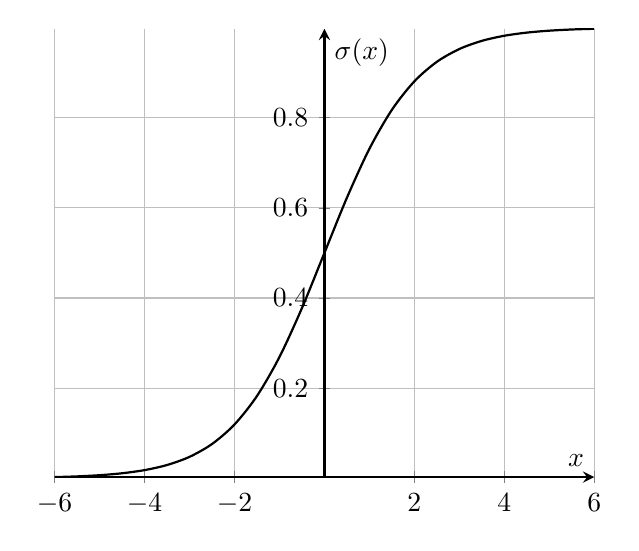
\begin{tikzpicture}
                \begin{axis}[ xlabel={$x$}, ylabel={$\sigma(x)$},
                    axis lines=middle, smooth , grid , thick, domain=-6:6]
                    \addplot[no marks]{1/(1+exp(-\x))};
                \end{axis}
            \end{tikzpicture}
            \vspace{2ex}
        \end{center}
        Com essa nota\'c\~ao, temos
        \begin{align*}
            p(h_i=1 | \v) &= \sigma\left(\sum_j W_{ji} v_j  + b_i\right).
        \end{align*}
        
    \end{solution}
    
    \item Use um argumento de simetria para mostrar que
    $$p(\v | \h) = \prod_i p(v_i | \h) \quad \text{ e }  \quad p(v_i = 1 | \h) = \frac{1}{1+\exp\left(-a_i-\sum_j W_{ij} h_j\right)}$$
    
    \begin{solution}
        Como $\v^\top \W \h$ \'e um escalar, temos $(\v^\top \W \h)^\top = \h^\top \W^\top \v =  \v^\top \W \h$, de modo que
        \begin{align}
            p(\v,\h) & \propto \exp\left( \v^\top \W \h + \a^\top\v + \b^\top\h \right) \\
            & \propto \exp\left( \h^\top \W^\top \v + \b^\top\h + \a^\top\v  \right).
        \end{align}
        Para derivar o resultado, notamos que $\v$ e $a$ agora ocupam o lugar de $\h$ e $b$ de antes, e que agora temos $\W^\top$ em vez de $\W$. Na Equa\'c\~ao \eqref{eq:hcondv-corrected}, substitu\'imos assim $h_i$ com $v_i$, $b_i$ com $a_i$, e $W_{ji}$ com $W_{ij}$ para obter $p(v_i = 1 | \h)$. Em termos da fun\'c\~ao sigm\'oide, temos
        $$ p(v_i=1 | \h) = \sigma\left(\sum_j W_{ij} h_j + a_i\right).$$
        
        Note que, embora $p(\v | \h)$ se fatorize, a marginal $p(\v)$
        geralmente n\~ao. A marginal $p(\v)$ pode aqui ser obtida em
        forma fechada at\'e sua constante de normaliza\'c\~ao.
        \begin{align}
            p(\v) & = \sum_{\h \in \{0,1\}^m} p(\v,\h) \\
            & = \frac{1}{Z} \sum_{\h \in \{0,1\}^m} \exp\left( \v^\top \W \h + \a^\top\v + \b^\top\h \right)\\
            & =  \frac{1}{Z}  \sum_{\h \in \{0,1\}^m} \exp\left( \sum_{ij} v_i h_j W_{ij} + \sum_i a_i v_i + \sum_j b_j h_j \right)\\
            & =  \frac{1}{Z}  \sum_{\h \in \{0,1\}^m} \exp\left( \sum_{j=1}^m h_j \left[\sum_i v_i W_{ij} + b_j\right] + \sum_i a_i v_i \right)\\
            & =  \frac{1}{Z}  \sum_{\h \in \{0,1\}^m} \prod_{j=1}^m \exp\left( h_j \left[\sum_i v_i W_{ij} + b_j\right] \right) \exp\left( \sum_i a_i v_i \right)\\
            & =  \frac{1}{Z} \exp\left( \sum_i a_i v_i \right) \sum_{\h \in \{0,1\}^m} \prod_{j=1}^m \exp\left( h_j \left[\sum_i v_i W_{ij} + b_j\right] \right) \\
            & =  \frac{1}{Z} \exp\left( \sum_i a_i v_i \right) \sum_{h_1, \ldots, h_m} \prod_{j=1}^m  \exp\left( h_j \left[\sum_i v_i W_{ij} + b_j\right] \right)
        \end{align}
        O mais importante \'e que cada termo no produto depende apenas de um \'unico $h_j$, de modo que, ao aplicar sequencialmente a lei distributiva, temos
        \begin{align}
            \sum_{h_1, \ldots, h_m} \prod_{j=1}^m  \exp\left( h_j \left[\sum_i v_i W_{ij} + b_j\right] \right)  =& \left[ \sum_{h_1, \ldots, h_{m-1}} \prod_{j=1}^{m-1}  \exp\left( h_j \left[\sum_i v_i W_{ij} + b_j\right] \right)\right] \cdot \nonumber \\
            &\sum_{h_m} \exp\left( h_m \left[\sum_i v_i W_{im} + b_m\right] \right)\\
            =& \ldots \nonumber \\
            =& \prod_{j=1}^m \left[\sum_{h_j} \exp\left( h_j \left[\sum_i v_i W_{ij} + b_j\right] \right)\right]
        \end{align}
        Como $h_j \in \{0,1\}$, obtemos
        \begin{align}
            \sum_{h_j} \exp\left( h_j \left[\sum_i v_i W_{ij} + b_j\right] \right) & = 1+ \exp\left(\sum_i v_i W_{ij} + b_j \right)
        \end{align}
        e assim
        \begin{align}
            p(\v) & = \frac{1}{Z}  \exp\left( \sum_i a_i v_i \right) \prod_{j=1}^m \left[1+ \exp\left(\sum_i v_i W_{ij} + b_j \right)\right].
        \end{align}
        Note que, na deriva\'c\~ao de $p(\v)$, n\~ao usamos a
        hip\'otese de que os vis\'iveis $v_i$ s\~ao bin\'arios. A mesma
        express\~ao seria obtida, portanto, se os vis\'iveis fossem definidos em
        outro espa\'co, e.g.\ os n\'umeros reais.
        
        Enquanto $p(\v)$ \'e escrita como um produto, $p(\v)$ n\~ao
        se fatoriza em termos que dependem de subconjuntos dos
        $v_i$. Pelo contr\'ario, todos os $v_i$ est\~ao presentes em todos os
        fatores. Como $p(\v)$ n\~ao se fatoriza, computar a constante de
        normaliza\'c\~ao $Z$ \'e custoso. Para vis\'iveis bin\'arios
        $v_i \in \{0,1\}$, $Z$ \'e igual a
        \begin{equation}
            Z = \sum_{\v \in \{0,1\}^n} \exp\left( \sum_i a_i v_i \right) \prod_{j=1}^m \left[1+ \exp\left(\sum_i v_i W_{ij} + b_j \right)\right]
        \end{equation}
        onde temos que somar sobre todas as $2^n$ configura\'c\~oes dos
        vis\'iveis $\v$. Isso \'e computacionalmente custoso, ou mesmo
        proibitivo se $n$ for grande ($2^{20} = 1048576,\, 2^{30}>
        10^9$). Note que diferentes valores de $a_i,b_i,W_{ij}$ resultam em
        diferentes valores de $Z$. (Esta \'e uma raz\~ao pela qual $Z$ \'e chamada de
        fun\'c\~ao de parti\'c\~ao quando os $a_i, b_i, W_{ij}$ s\~ao par\^ametros livres.)
        
        \'E instrutivo escrever $p(\v)$ no dom\'inio logar\'itmico,
        \begin{align}
            \log p(\v) & = -\log Z + \sum_{i=1}^n a_i v_i + \sum_{j=1}^m \log\left[1+ \exp\left(\sum_i v_i W_{ij} + b_j \right)\right],
        \end{align}
        e introduzir a n\~ao linearidade $f(u)$,
        \begin{align}
            f(u) & = \log\left[ 1+\exp(u) \right],
        \end{align}
        que \'e chamada de fun\'c\~ao softplus e est\'a plotada abaixo. A fun\'c\~ao softplus \'e uma aproxima\'c\~ao suave de $\max(0,u)$, veja e.g.\ \url{https://en.wikipedia.org/wiki/Rectifier_(neural_networks)}
        \begin{center}
            \vspace{3ex}
            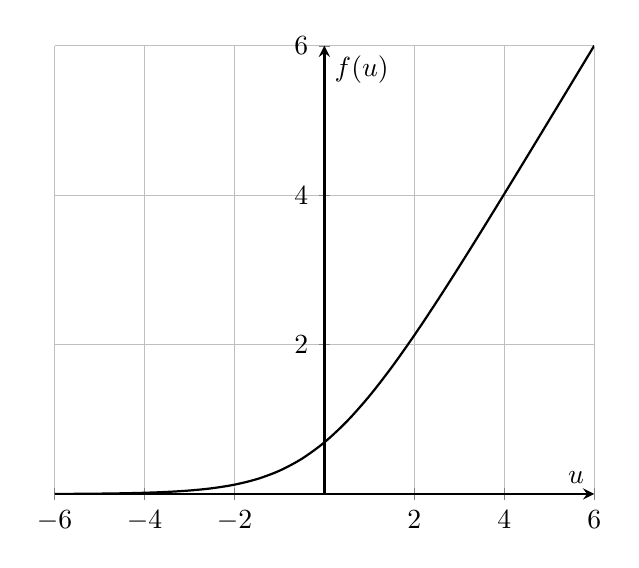
\begin{tikzpicture}
                \begin{axis}[ xlabel={$u$}, ylabel={$f(u)$},
                    axis lines=middle, smooth , grid , thick, domain=-6:6]
                    %          \draw[->] (-5,0) -- (5,0) node[right] {$x$};
                    %          \draw[->] (0,0) -- (0,1.5) node[above] {$\sigma(x)$};
                    \addplot[no marks]{ln(1+exp(\x))};
                    %\addplot[no marks, red]{max(\x,0)};
                \end{axis}
            \end{tikzpicture}
        \end{center}
        Com a fun\'c\~ao softplus $f(u)$, podemos escrever $\log p(\v)$ como
        \begin{align}
            \log p(\v) & = \log Z + \sum_{i=1}^n a_i v_i + \sum_{j=1}^m f\left(\sum_i v_i W_{ij} + b_j \right).
        \end{align}
        O par\^ametro $b_j$ desempenha o papel de um limiar como mostrado na
        figura abaixo. Os termos $f\left(\sum_i v_i W_{ij} + b_j
        \right)$ podem ser interpretados em termos de detec\'c\~ao de caracter\'isticas (features). A
        soma $\sum_i v_i W_{ij}$ \'e o produto interno entre $\v$ e
        a $j$-\'esima coluna de $\W$, e o produto interno \'e maior se
        $\v$ for igual \`a $j$-\'esima coluna. Podemos, assim, considerar as colunas
        de $\W$ como moldes de caracter\'isticas (feature-templates), e o $f\left(\sum_i v_i
        W_{ij} + b_j \right)$ uma forma de medir quanto de cada caracter\'istica
        est\'a presente em $\v$.
        
        Al\'em disso, $\sum_i v_i W_{ij} +b_j$ tamb\'em \'e a entrada para a
        fun\'c\~ao sigm\'oide ao computar $p(h_j=1 | \v)$. Assim, a
        probabilidade condicional de $h_j$ ser um, i.e.\ ``ativa'',
        pode ser considerada um indicador da presen\'ca da
        $j$-\'esima caracter\'istica ($j$-\'esima coluna de $\W$) na entrada $\v$.
        
        Se $v$ for tal que $\sum_i v_i W_{ij} +b_j$ for grande para muitos
        $j$, i.e.\ se muitas caracter\'isticas forem detectadas, ent\~ao $f\left(\sum_i
        v_i W_{ij} + b_j \right)$ ser\'a n\~ao nulo para muitos $j$, e
        $\log p(\v)$ ser\'a grande.
        
        
        \begin{center}
            \vspace{3ex}
            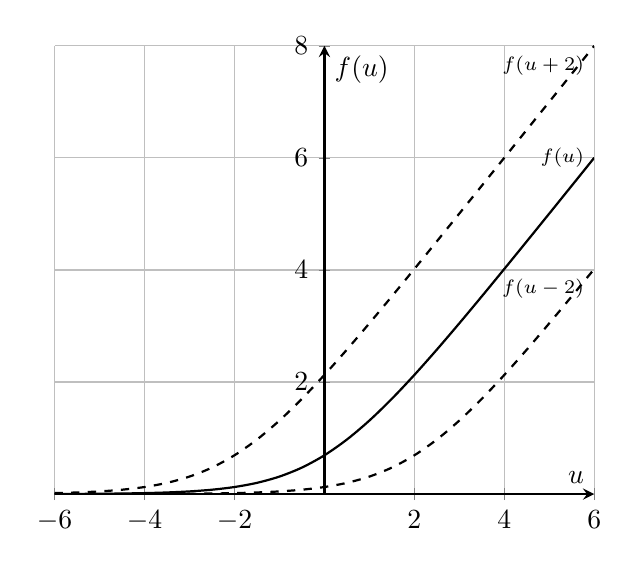
\begin{tikzpicture}
                \begin{axis}[ xlabel={$u$}, ylabel={$f(u)$},
                    axis lines=middle, smooth , grid , thick, domain=-6:6]
                    %          \draw[->] (-5,0) -- (5,0) node[right] {$x$};
                    %          \draw[->] (0,0) -- (0,1.5) node[above] {$\sigma(x)$};
                    \addplot[no marks]{ln(1+exp(\x))} node[left]{\scriptsize$f(u)$};
                    \addplot[no marks, dashed]{ln(1+exp(\x+2))} node[below left]{\scriptsize $f(u+2)$};
                    \addplot[no marks, dashed]{ln(1+exp(\x-2))} node[below left]{\scriptsize $f(u-2)$};
                    %\addplot[no marks, red]{max(\x,0)};
                \end{axis}
            \end{tikzpicture}
        \end{center}
        
        
    \end{solution}
    
    
    
\end{exenumerate}



\ex{Modelos ocultos de Markov e mudan\'ca de medida}

Considere o seguinte grafo n\~ao direcionado para um modelo oculto de Markov onde os $y_i$ correspondem a vari\'aveis observadas (vis\'iveis) e os $x_i$ a vari\'aveis n\~ao observadas (ocultas/latentes).

\begin{center}
    \scalebox{1}{
        \begin{tikzpicture}[ugraph]
            \node[cont] (x1) at (0,2) {$x_1$};
            \node[cont] (x2) at (2,2) {$x_2$};
            \node[cont] (x3) at (4,2) {$x_3$};
            \node       (a) at (6,2) {};
            \node       (b) at (7,2) {$\ldots$};
            \node       (c) at (7,0) {$\ldots$};
            \node       (d) at (8,2) {};
            \node[cont] (x4) at (10,2) {$x_t$};
            \node[cont] (y1) at (0,0) {$y_1$};
            \node[cont] (y2) at (2,0) {$y_2$};
            \node[cont] (y3) at (4,0) {$y_3$};
            \node[cont] (y4) at (10,0) {$y_t$};
            \draw(x1)--(y1);\draw(x2)--(y2);\draw(x3)--(y3);\draw(x4)--(y4);
            \draw(x1)--(x2);\draw(x2)--(x3);\draw(x3)--(a);\draw(d)--(x4);
    \end{tikzpicture}}
\end{center}

O grafo implica a seguinte fatoriza\'c\~ao
\begin{equation}
    p( x_1, \ldots, x_t,y_1, \ldots, y_t) \propto \phi_1^y(x_1, y_1) \prod_{i=2}^t \phi_i^x(x_{i-1}, x_i) \phi_i^y(x_i, y_i),
\end{equation}
onde as $\phi_i^x$ e $\phi_i^y$ s\~ao fatores n\~ao-negativos.

Consideremos a situa\'c\~ao onde $\prod_{i=2}^t \phi^x_i(x_{i-1}, x_i)$ \'e igual a
\begin{equation}
    f(\x) = \prod_{i=2}^t \phi^x_i(x_{i-1}, x_i) = f_1(x_1) \prod_{i=2}^t f_i(x_i|x_{i-1}),
\end{equation}
com $\x=(x_1, \ldots, x_t)$ e onde os $f_i$ s\~ao fdps (condicionais). Temos portanto
\begin{align}
    p(x_1, \ldots, x_t, y_1, \ldots, y_t) \propto f_1(x_1) \prod_{i=2}^t f_i(x_i|x_{i-1}) \prod_{i=1}^t \phi_i^y(x_i, y_i).
    \label{eq:Markov-model-joint-def-corrected}
\end{align}

\begin{exenumerate}
    
    \item Forne\'ca uma express\~ao fatorizada para $ p(x_1, \ldots, x_t | y_1, \ldots, y_t)$
    
    \begin{solution}
        Para valores fixos (observados) dos $y_i$, $p(x_1, \ldots, x_t |
        y_1, \ldots, y_t)$ se fatoriza como
        \begin{align}
            p(x_1, \ldots, x_t | y_1, \ldots, y_t) \propto f_1(x_1) g_1(x_1)
            \prod_{i=2}^t f_i(x_i|x_{i-1}) g_i(x_i).
        \end{align}
        onde $g_i(x_i)$ \'e $\phi^y_i(x_i,y_i)$ para um valor fixo de $y_i$.
    \end{solution}
    
    \item Desenhe o grafo n\~ao direcionado para $p(x_1, \ldots, x_t | y_1, \ldots, y_t)$
    \begin{solution}
        O condicionamento corresponde \`a remo\'c\~ao de n\'os de um grafo n\~ao
        direcionado. Temos portanto a seguinte cadeia de Markov para $p(x_1, \ldots,
        x_t | y_1, \ldots, y_t)$.
        
        \begin{center}
            \scalebox{1}{
                \begin{tikzpicture}[ugraph]
                    \node[cont] (x1) at (0,0) {$x_1$};
                    \node[cont] (x2) at (2,0) {$x_2$};
                    \node[cont] (x3) at (4,0) {$x_3$};
                    \node       (a) at (6,0) {};
                    \node       (b) at (7,0) {$\ldots$};
                    \node       (d) at (8,0) {};
                    \node[cont] (x4) at (10,0) {$x_t$};
                    \draw(x1)--(x2);\draw(x2)--(x3);\draw(x3)--(a);\draw(d)--(x4);
                \end{tikzpicture}
            }
        \end{center}
        
    \end{solution}
    
    \item Mostre que se $\phi_i^y(x_i, y_i)$ for igual \`a fdp condicional de
    $y_i$ dado $x_i$, i.e.\ $p(y_i|x_i)$, a marginal $p(x_1, \ldots, x_t)$,
    obtida integrando em rela\'c\~ao a $y_1, \ldots, y_t$ a partir de
    \eqref{eq:Markov-model-joint-def-corrected}, \'e igual a $f(\x)$.
    
    \begin{solution}
        Nesse cenário, todos os fatores em \eqref{eq:Markov-model-joint-def-corrected}
        s\~ao fdps condicionais e estamos lidando com um modelo gr\'afico
        direcionado que se fatoriza como
        \begin{equation}
            p(x_1, \ldots, x_t, y_1, \ldots, y_t) = f_1(x_1) \prod_{i=2}^t f_i(x_i|x_{i-1}) \prod_{i=1}^t p(y_i|x_i).
        \end{equation}
        Ao integrar sobre os $y_i$, temos
        \begin{align}
            p(x_1, \ldots, x_t) &= \int p(x_1, \ldots, x_t, y_1, \ldots, y_t) \ud y_1 \ldots \ud y_t\\
            & = f_1(x_1) \prod_{i=2}^t f_i(x_i|x_{i-1}) \int \prod_{i=1}^t p(y_i|x_i) \ud y_1 \ldots \ud y_t\\
            & = f_1(x_1) \prod_{i=2}^t f_i(x_i|x_{i-1}) \prod_{i=1}^t \underbrace{\int  p(y_i|x_i) \ud y_i}_{1}\\
            & = f_1(x_1) \prod_{i=2}^t f_i(x_i|x_{i-1})\\
            & = f(\x)
        \end{align}
        
    \end{solution}
    
    
    \item Calcule a constante de normaliza\'c\~ao para $p(x_1, \ldots, x_t | y_1, \ldots, y_t)$ e expresse-a como uma esperan\'ca sobre $f(\x)$.
    \begin{solution}
        Com
        \begin{align}
            p(x_1, \ldots, x_t | y_1, \ldots, y_t) \propto f_1(x_1) \prod_{i=2}^t f_i(x_i|x_{i-1}) \prod_{i=1}^t \phi_i^y(x_i, y_i).
        \end{align}
        A constante de normaliza\'c\~ao \'e dada por
        \begin{align}
            Z & = \int f_1(x_1) \prod_{i=2}^t f_i(x_i|x_{i-1})\prod_{i=1}^t g_i(x_i) \ud x_1 \ldots \ud x_t\\
            & = \E_f\left [\prod_{i=1}^t g_i(x_i) \right]
        \end{align}
        Como podemos usar amostragem ancestral para amostrar de $f$, a
        esperan\'ca acima pode ser facilmente computada via amostragem.
        
    \end{solution}
    
    \item Expresse a esperan\'ca de uma fun\'c\~ao de teste $h(\x)$ em rela\'c\~ao
    a $p(x_1, \ldots, x_t | y_1, \ldots, y_t)$ como uma esperan\'ca reponderada
    com respeito a $f(\x)$.
    
    \begin{solution}
        
        Por defini\'c\~ao, a esperan\'ca sobre uma fun\'c\~ao de teste $h(\x)$ \'e
        \begin{align}
            \E_{p(x_1, \ldots, x_t | y_1,
                \ldots, y_t)}[ h(\x) ] & = \frac{1}{Z} \int h(\x) f_1(x_1) \prod_{i=2}^t f(x_i|x_{i-1})\prod_{i=1}^t g_i(x_i) \ud x_1 \ldots \ud x_t\\
            & = \frac{\E_f \left[ h(\x) \prod_i g_i(x_i) \right]}{\E_f\left [\prod_i g_i(x_i) \right]}
        \end{align}
        Tanto o numerador quanto o denominador podem ser aproximados usando
        amostras de $f$.
        
        Como os $g_i(x_i) = \phi_i^y(x_i,y_i)$ envolvem as vari\'aveis observadas
        $y_i$, isso tem uma interpreta\'c\~ao interessante: Podemos pensar que
        temos dois modelos para $\x$: $f(\x)$ que n\~ao envolve as
        observa\'c\~oes e $p(x_1, \ldots, x_t | y_1,\ldots, y_t)$ que
        envolve. Note, por\'em, que a menos que $\phi_i^y(x_i, y_i)$ seja a
        fdp condicional $p(y_i|x_i)$, $f(\x)$ \emph{n\~ao} \'e a marginal
        $p(x_1, \ldots, x_t)$ que voc\^e obteria integrando os
        $y$'s do modelo conjunto. Podemos ent\~ao geralmente pensar que \'e uma
        distribui\'c\~ao base que foi ``melhorada'' por uma mudan\'ca de medida em nossa express\~ao para
        $p(x_1, \ldots, x_t| y_1,\ldots, y_t)$. Se $\phi_i^y(x_i, y_i)$ for
        a fdp condicional $p(y_i|x_i)$, a mudan\'ca de medida
        corresponde a ir da priori para a posteriori por
        multiplica\'c\~ao com a verossimilhan\'ca (os termos $g_i$).
        
        A partir da express\~ao para a esperan\'ca, podemos ver que o
        ``melhoramento'' leva a uma correspondente introdu\'c\~ao de pesos na
        esperan\'ca que dependem via $g_i$ das observa\'c\~oes. Isso
        pode ser particularmente bem visto quando aproximamos a esperan\'ca como
        uma m\'edia amostral sobre $n$ amostras $\x^{(k)} \sim f(\x)$:
        \begin{align}
            \E_{p(x_1, \ldots, x_t | y_1, \ldots, y_t)}[ h(\x) ] & \approx \sum_{k=1}^n W^{(k)} h(\x^{(k)})\\
            W^{(k)} & =  \frac{w^{(k)}}{\sum_{k=1}^n  w^{(k)}}\\
            w^{(k)} & =  \prod_i g_i(x^{(k)}_i)
        \end{align}
        onde $x^{(k)}_i$ \'e a $i$-\'esima dimens\~ao do vetor $\x^{(k)}$.
    \end{solution}
    
\end{exenumerate}